\documentclass[sigconf,authordraft]{acmart}
\usepackage{tikz}
\usepackage{todonotes}
\usetikzlibrary{arrows}

\newcommand{\den}[2][]{
\left\llbracket#2\right\rrbracket^{#1}
}
\newcommand{\low}[1]{
\left\lfloor#1\right\rfloor
}
\newcommand{\denml}[1]{
  \den[ml]{#1}
}
\newcommand{\denev}[1]{
  \den[ev]{#1}
}

\newcommand{\squash}{\itemsep=0pt\parskip=0pt}
\newcommand{\uavam}{\textsf{UAVAM}}
\newcommand{\useram}{\textsf{UserAM}}
\newcommand{\platam}{\textsf{PlatformAM}}
\newcommand{\selam}{\textsf{seL4AM}}
\newcommand{\uboot}{\textsf{UBOOT}}
\newcommand{\duhk}{\textsf{DUHK}}
\newcommand{\M}[1]{\ensuremath{M_{\mathsf{#1}}}}
\newcommand{\E}[1]{\ensuremath{E_{\mathsf{#1}}}}
\newcommand{\R}[1]{\ensuremath{R_{\mathsf{#1}}}}
\newcommand{\sign}[2]{\ensuremath{\{#1\}_{#2^{-1}}}}

%% The article template's documentation, available at
%% \url{https://www.acm.org/publications/proceedings-template}, has a
%% complete explanation of these commands and tips for their effective
%% use.

\setcopyright{acmcopyright}
\copyrightyear{2020}
\acmYear{2020}
\acmDOI{0000}

%% These commands are for a PROCEEDINGS abstract or paper.
\acmConference[Attestation Negotiation]{Working Paper on Attestation
  Negotiation}{20 January, 2020}{Lawrence, KS}
\acmBooktitle{No Book}
\acmPrice{0.00}
\acmISBN{0000}

%%\acmSubmissionID{123-A56-BU3}


\begin{document}

\title{Negotiating Attestation Protocols}

\author{Anna Fritz}
\email{arfritzz@ku.edu}
\author{Perry Alexander}
\orcid{0000-0002-5387-9157}
\email{palexand@ku.edu}
\affiliation{%
  \institution{ITTC - The University of Kansas}
  \streetaddress{2335 Irving Hill Rd}
  \city{Lawrence}
  \state{Kansas}
  \country{USA}
  \postcode{66045}
}

\renewcommand{\shortauthors}{Fritz and Alexander}

\begin{abstract}
  Abstract goes here
\end{abstract}

%%
%% The code below is generated by the tool at http://dl.acm.org/ccs.cfm.
%% Please copy and paste the code instead of the example below.
%%
\begin{CCSXML}
<ccs2012>
 <concept>
  <concept_id>10010520.10010553.10010562</concept_id>
  <concept_desc>Computer systems organization~Embedded systems</concept_desc>
  <concept_significance>500</concept_significance>
 </concept>
 <concept>
  <concept_id>10010520.10010575.10010755</concept_id>
  <concept_desc>Computer systems organization~Redundancy</concept_desc>
  <concept_significance>300</concept_significance>
 </concept>
 <concept>
  <concept_id>10010520.10010553.10010554</concept_id>
  <concept_desc>Computer systems organization~Robotics</concept_desc>
  <concept_significance>100</concept_significance>
 </concept>
 <concept>
  <concept_id>10003033.10003083.10003095</concept_id>
  <concept_desc>Networks~Network reliability</concept_desc>
  <concept_significance>100</concept_significance>
 </concept>
</ccs2012>
\end{CCSXML}

\ccsdesc[500]{Computer systems organization~Embedded systems}
\ccsdesc[300]{Computer systems organization~Redundancy}
\ccsdesc{Computer systems organization~Robotics}
\ccsdesc[100]{Networks~Network reliability}

\keywords{TBD}

\maketitle

\section{Introduction}

\citet{Martin:08:The-ten-page-in} defines trust as unambiguous
identification, unhindered operation, and direct observation of good
behavior or indirect observation by a trusted third party.  Semantic
remote attestation~\cite{Haldar:04:Semantic-Remote} is a technique by
which a target provides evidence used to establish trust in its
execution.  Shown in figure~\ref{fig:architecture-fig} and
\emph{appraiser} makes a request ($r:R$) of a \emph{target} than in
turn generates and returns evidence ($e:E$) that is appraised to
determine trust.

\begin{figure}[hbtp]
  \centering
  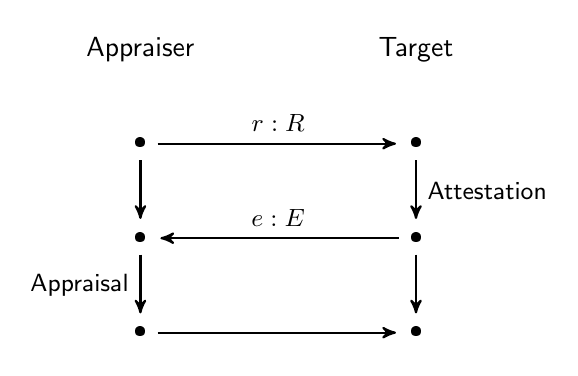
\begin{tikzpicture}[->,>=stealth',shorten >=1pt,auto,node distance=1.2cm,
  thick,main node/.style={rectangle,%fill=blue!20,draw,
    font=\sffamily,minimum height=2mm,minimum width=2mm},
  io node/.style={rectangle,
    font=\sffamily,minimum height=5mm,minimum width=10mm}]

  \node[main node] (APPTITLE) {Appraiser};
  \node[main node] (TARTITLE) [node distance=3.5cm, right of=APPTITLE] {Target};
  \node[main node] (SREQ) [below of=APPTITLE] {\textbullet};
  \node[main node] (RREQ) [below of=TARTITLE] {\textbullet};
  \node[main node] (REV) [below of=SREQ] {\textbullet};
  \node[main node] (SEV) [below of=RREQ] {\textbullet};
  \node[main node] (APP) [below of=REV] {\textbullet};
  \node[main node] (NONE) [below of=SEV] {\textbullet};
    
  \path[every node/.style={font=\sffamily\small, fill=white,inner sep=1pt}]
    (SREQ) edge node[above=1mm] {$r:R$} (RREQ)
    (SEV) edge node[above=1mm] {$e:E$} (REV)
    (APP) edge (NONE)
    (SREQ) edge (REV)
    (RREQ) edge node[right=1mm] {Attestation} (SEV)
    (SEV) edge (NONE)
    (REV) edge node[left=1mm] {Appraisal} (APP)
    ;
\end{tikzpicture}

%%% Local Variables: 
%%% mode: latex
%%% TeX-master: "negotiation20"
%%% End:

  \caption[Attestation architecture]{Remote attestation architecture
    showing an \emph{appraiser} making an attestation request of a
    \emph{target}.}
  \Description{Remote attestation basic architecture.}
  \label{fig:architecture-fig}
\end{figure}

\citet{Coker::Principles-of-R,Coker:08:Attestation:-Ev} define a
remote attestation model where a target executes an \emph{attestation
  protocol} that gathers evidence and generates meta-evidence for
appraisal.  The protocol sequences the execution of attestation
services that perform measurement, generate cryptographic signatures,
and make requests of other systems. These protocols are executed by an
\emph{attestation manager} associated with the appraiser or target.

Figure~\ref{fig:sequence-fig} illustrates the process of negotiating
and executing an attestation protocol.  An appraiser and target first
establish a security association that identifies appraiser and target,
sets up secure communication and establishes a security domain
providing context for negotiation.  The appraiser then sends a
request to the target describing the evidence and meta-evidence it
needs for appraisal.  The target produces a proposal consisting of a
protocol set that responds to the request while obeying the target's
local policy.  The appraiser chooses a protocol from the proposal that
the target then executes.  The resulting evidence is returned to the
appraiser and evaluated to determine trust.

%% just decribe whats in it. domain which defines vocabulary 

It is important to note that in order to begin the negotiation procedure,
a security association (SA) must be established. The security association is essential as it authorizes the parties to communicate under the same vocabulary. More precisely, a SA  establishes identification, keys, security labels, and  a domain of interpretation. It could also include details pertaining to situational awareness and its lifetime. To enstanciate the SA, an appriaser sends a request to the target where, through ISAKMP, the target responds with the certificate validating the security association. Communcation between the two parties can then occur under a common domain of interpretation.   

The negotiation of an attestation protocol satisfying the
requirements of the appraiser and restrictions of the target is our
objective here.  Following we will formally define a negotiation
process, define properties of an ideal protocol, and show that the
negotiation process produces ideal protocols.  We will then
instantiate the model for several systems to provide examples of its use.

\section{Attestation Protocols}

An attestation protocol is formally a sequence of attestation actions
that can include gathering evidence in sequence and parallel,
generating cryptographic signatures, and requesting attestation
results from other attestation managers.  Our representation for such
protocols uses Copland~\citep{Ramsdell:2019aa} which provides a
convenient language for modeling and execution as well as a formal
semantics for verification.

\todo[inline]{section should continue and define/describe Copland
  protocols.  Important concepts are ASPs, protocols, evidence and
  meta-evidence}

\section{Protocol Negotiation}

For the purposes of his discussion we will assume the establishment of
a security association between appraiser and target and begin with the
appraiser sending a request to the target.  We define $A$ as the type
of appraisers and $T$ the type of targets.  $R$ is the type of
attestation requests that define the needs of the appraiser.  $P$ is
the type of protocols represented as Copland phrases.  $E$ is the type
of evidence generated by protocol execution.

Ideally the appraiser $a:A$ makes a request $r:R$ of some target
$t:T$, a protocol $p:P$ is selected and executed buy $t$ returning
evidence $e:E$ for evaluation by $a$.  Selection of $p$ is achieved by
finding the ``best'' protocol that satisfies the needs of the
appraiser while respecting the privacy of the target. The notion of
``best'' is situationally dependent and can change for different
attestation scenarios, targets and appraisers.  Furthermore, the
preferences and policies of targets and appraisers are not and should
not be globally known.  Thus, negotiation between $a$ and $t$ is
essential for finding a ``best'' protocol.  

Figure~\ref{fig:sequence-fig} graphically shows the negotiation
process for finding a best $p$ given a request $r$ and a collection of
available protocols, $P$.

We define $\langle P \rangle$ as vectors of protocols
representing \emph{proposals}.  When an appraiser makes a request,
the target returns some $q:\langle P \rangle$ whose protocols fully or
partially satisfy the request. The target chooses and orders
$q:\langle P\rangle$ by examining evidence produced by executing
protocols defined by Copland's evidence semantics $\mathcal{E}$.

Two factors influence the production of $p$.  The target's \emph{local
policy} defines limits on the evidence it will provide.  Local policy 
$\pi : A\times E$ is a relation among appraisers and evidence.
$(a,e)\in\pi$ implies that appraiser $a$ has permission to receive
evidence $e$.  Thus, $\{e:E\mid (a,e)\in\pi\}$ is the evidence set a target
can return to $a$.

The target's negotiation policy defines an ordering over evidence and
indirectly an ordering over protocols.  The partially ordered set
$(E,\preceq)$ defines the target's preference for one evidence set
over another. $e_1\preceq e_2$ expresses a preference for $e_2$ over
$e_1$.  Taken further, if $(E,\preceq,\top,\bot)$ defines a lattice,
then $E$ and every subset of $E$ has one or more maxima.  Those maxima
define best or most preferred evidence.

Combining a request, local policy, and evidence preference results in
a lattice of evidence satisfying the request:

\[(\{e:E\mid (a,e)\in\pi_T\},\preceq_T,\top_T,\bot_T)\]

If $\mathcal{E}[\![p]\!]=e$ for some protocol $p$ then a similar
lattice for protocols results:

\[(\{p:P\mid (a,\mathcal{E}[\![p]\!]=e)\in\pi_T\},\preceq_T,\top_T,\bot_T)\]

\todo[inline]{stopped here for the evening.  what's above tries to
  reflect our discussions, but is not there yet.  several things need
  to be decided.  Also some redundant stuff follows.}

Elements of a proposal $\langle P\rangle$ are generated by
$(\mathsf{map}\; \mathcal{E}\; \langle P\rangle)$ where $\mathcal{E}$
is the Copland evidence semantics defined by \citet{Ramsdell:2019aa}.
Thus, a proposal can be mapped onto the various evidence that each
protocol produces.

Figure~\ref{fig:sequence-fig} defines the process of protocol
negotiation and execution.  $r:R$ is sent from appraiser to
target.  The target responds with a $q:\langle P\rangle$  defining potential
protocols.  The appraiser chooses one protocol, $p:P$, by direct selection and
instantiation of a parameterized protocol.  That protocol is then
executed by the target and evidence, $e:E$, returned to the appraiser.  The
evidence is then appraised to determine trust.

\begin{figure}[hbtp]
  \centering
  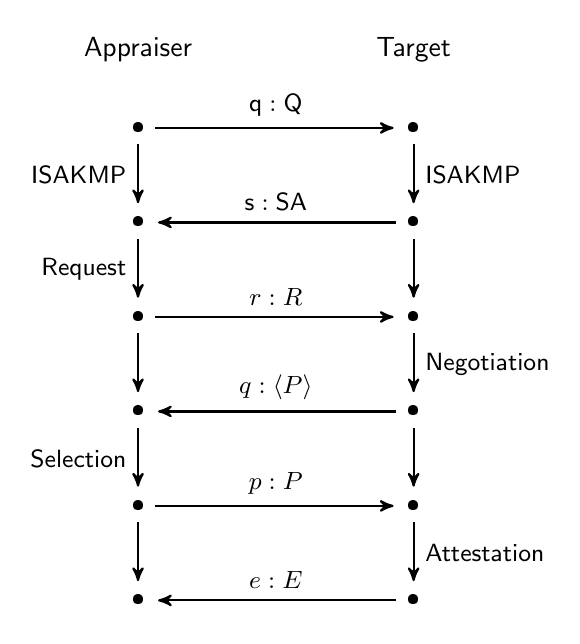
\begin{tikzpicture}[->,>=stealth',shorten >=1pt,auto,node distance=1.2cm,
  thick,main node/.style={rectangle,%%fill=blue!20,draw,
    font=\sffamily,minimum height=2mm,minimum width=2mm}]


  \node[main node] (RQ) {\textbullet};
  \node[main node] (SA) [below of=RQ] {\textbullet};
  \node[main node] (NM) [below of=SA] {\textbullet};
  \node[main node] (AM) [below of=NM] {\textbullet};
  \node[main node] (CP) [below of=AM] {\textbullet};
  \node[main node] (HW) [below of=CP] {\textbullet};
%%  \node[main node] (AP) [below of=HW] {\textbullet};
  \node[main node] (HWE) [node distance=3.5cm, right of=HW] {\textbullet};
  \node[main node] (CPE) [node distance=3.5cm, right of=CP] {\textbullet};
  \node[main node] (AME) [node distance=3.5cm, right of=AM] {\textbullet};
  \node[main node] (NME) [node distance=3.5cm, right of=NM] {\textbullet};
  \node[main node] (SAE) [node distance=3.5cm, right of=SA] {\textbullet};  
  \node[main node] (RQE) [node distance=3.5cm, right of=RQ] {\textbullet};  
  \node[main node] (IN) [node distance=1.0cm, above of=RQ] {Appraiser};
  \node[main node] (OUT) [node distance=1.0cm, above of=RQE] {Target};
    

  \path[every node/.style={font=\sffamily\small, fill=white,inner sep=1pt}]
    (RQ) edge node[above=1mm] {$\mathsf{q:Q}$} (RQE)
    (SAE) edge node[above=1mm] {$\mathsf{s:SA}$} (SA)
    (NM) edge node[above=1mm] {$r:R$} (NME)
    (AME) edge node[above=1mm] {$q:\langle P \rangle$} (AM)
    (CP) edge node[above=1mm] {$p:P$} (CPE)
    (HWE) edge node[above=1mm] {$e:E$} (HW)
    (RQ) edge node[left=1mm] {ISAKMP} (SA)
    (RQE) edge node[right=1mm] {ISAKMP} (SAE)
    (SA) edge node[left=1mm] {Request} (NM)
    (SAE) edge node[right=1mm] {} (NME)
    (NM) edge node[left=1mm] {} (AM)
    (NME) edge node[right=1mm] {Negotiation} (AME)
    (AM) edge node[left=1mm] {Selection} (CP)
    (AME) edge node[right=1mm] {} (CPE)
    (CP) edge node[left=1mm] {} (HW)
    (CPE) edge node[right=1mm] {Attestation} (HWE)
%%    (HW) edge node[left=1mm] {Appraisal} (AP)
    ;
\end{tikzpicture}

%%% Local Variables: 
%%% mode: latex
%%% TeX-master: "negotiation20"
%%% End:

  \caption[Attestation process]{Attestation process.}
  \Description{Attestation sequence.}
  \label{fig:sequence-fig}
\end{figure}

Figure \ref{fig:certification-fig}.

\begin{figure}[hbtp]
  \centering
  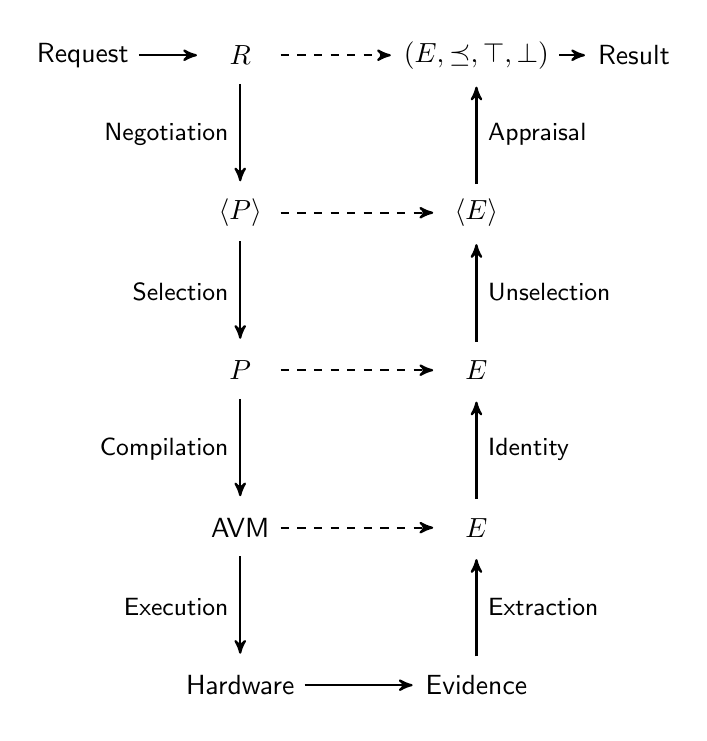
\begin{tikzpicture}[->,>=stealth',shorten >=1pt,auto,node distance=2.0cm,
  thick,main node/.style={rectangle,%%fill=blue!20,draw,
    font=\sffamily,minimum height=7mm,minimum width=10mm}]

  \node[main node] (Request) {$R$};
  \node[main node] (Proposal) [below of=Request] {$\langle P\rangle $};
  \node[main node] (Phrase) [below of=Proposal] {$P$};
  \node[main node] (AttInt) [below of=Phrase] {$\mathsf{AVM}$};
  \node[main node] (Hardware) [below of=AttInt] {Hardware};
  \node[main node] (Bits) [node distance=3.0cm, right of=Hardware] {Evidence};
  \node[main node] (VME) [node distance=3.0cm, right of=AttInt] {$E$};
  \node[main node] (Evidence) [node distance=3.0cm, right of=Phrase] {$E$};
  \node[main node] (EvidenceVec) [node distance=3.0cm, right of=Proposal] {$\langle E\rangle$};
  \node[main node] (Result) [node distance=3.0cm, right of=Request]
  {$(E,\preceq,\top,\bot)$};
  \node[main node] (IN) [node distance=2.0cm, left of=Request] {Request};
  \node[main node] (OUT) [node distance=2.0cm, right of=Result] {Result};
    

  \path[every node/.style={font=\sffamily\small, fill=white,inner sep=1pt}]
    (IN) edge (Request)
    (Request) edge node[left=1mm] {Negotiation} (Proposal)
    (Proposal) edge node[left=1mm] {Selection} (Phrase)
    (Phrase) edge node[left=1mm] {Compilation} (AttInt)
    (AttInt) edge node[left=1mm] {Execution} (Hardware)
    (Hardware) edge node[below=1mm] {} (Bits)
    (AttInt) edge [dashed] node[below=1mm] {} (VME)
    (Phrase) edge [dashed] node[below=1mm] {} (Evidence)
    (Proposal) edge [dashed] node[below=1mm] {} (EvidenceVec)
    (Request) edge [dashed] node[below=1mm] {} (Result)
    (Bits) edge node[right=1mm] {Extraction} (VME)
    (VME) edge node[right=1mm] {Identity} (Evidence)
    (Evidence) edge node[right=1mm] {Unselection} (EvidenceVec)
    (EvidenceVec) edge node[right=1mm] {Appraisal} (Result)
    (Result) edge (OUT)
    ;
\end{tikzpicture}

%%% Local Variables: 
%%% mode: latex
%%% TeX-master: "negotiation20"
%%% End:

  \caption[Attestation process]{Certification figure.}
  \Description{Certification figure.}
  \label{fig:certification-fig}
\end{figure}

\todo[inline] {do we have semantics for unselection? }
\todo[inline] {selection and unselection together define a Galios
  connection.  selection is concretization and unselection is abstraction.}

\section{Negotiation Verification}

Knowing that a request $r:R$ produces evidence, we can send a request through the attestation manager to generate all possible pieces of evidence. From that resulting vector of evidence, a situationally dependent ordering will be imposed and one piece of evidence will be deemed ``best''. This ``best'' piece of evidence represents the top of the lattice. As seen in figure 3, this procedure is described using the top arrow where the $r:R$ generates a vector of evidence. We will then move backwards through the certification figure to enforce an ordering over the possible pieces of evidence $\langle E \rangle$, undoing appraisal. We can take the ordering of evidence and order the possible protocols generated from the request. This repensents the appraiser's ordering of protocols, creating the appraiser's lattice. After the request is sent, we can then compare the appraiser's protocol ordering to the target's proposal. The protocol selected for attestation will be the one that is ``best'' for the appraiser and that is included in the target's proposal.      

\section{Conclusions}

We have presented a model for negotiating attestation protocols that
both meet local policy requirements while producing evidence
satisfying appraiser requirements.

\nocite{Coker::Principles-of-R,Ramsdell:2019aa,Petz:2019aa,Davey:02:Introduction-to}

\bibliographystyle{ACM-Reference-Format}
\bibliography{sldg}

\end{document}

